\section{Motivation and related work}
\label{sec:motive}

\textbf{Motivating result 1:  Process-Level Isolation Can't Cut It.}
Our first question was what isolation and execution mechanisms could support
our aggressive goal of 10$\mu{}s$ remote function invocation latency, while
having more microservices running than there are cores on a server.
Because of the popularity of container-based approaches (which use processes
plus some additional system call restrictions), we first measured the time
to locally invoke a simple process via Unix IPC.  This result provides
a lower bound on the invocation latency for a remote process over the network.
\solb{This is a stronger claim than I was trying to make:\ I merely claimed it was a
lower bound on the local invocation latency.  Throughout this section I've been
assuming we're solely talking about local numbers, albeit motivated by the 20us
network number that we're trying to stay *comfortably* below.}
The results are shown in Figure~\ref{fig:motive}.

The top (very slow) blue line shows the time to fork/exec a process upon receipt
of a new function invocation.  At over 1ms, this solution clearly does not
suffice.  Next is the time required to dynamically load a library into a shared
worker process.  This time is better, but is still an order of magnitude over
our target.  The green line shows the time it takes to send a UDP packet
\emph{locally} to an already-forked (but blocked) process.  The bottom
line shows the latency of invoking a true function call as a preloaded dynamic
library in a shared worker process.  From this, we observe that the
``per-process'' model, wherein a cold start corresponds to forking a new
process, and a warm start to unblocking it via I/O, has latencies that are
generally outside of our target range.

Because of this high latency, ew eschew the process-per-microservice model.
We instead propose
collecting groups of microservices into shared \textbf{worker processes},
each responsible for performing all the work assigned to a given CPU core.  We can
ensure that these will always be running, so the cold start case now only requires
loading user code into an existing process (a few tens of microseconds instead
of milliseconds).  We do this by packaging user
microservices as shared object files and using the dynamic linker/loader's
\texttt{dlopen()} interface.  Because each worker owns its cores, they can spend any
(rare) time between user tasks polling for the next job to arrive, so a warm start
simply involves flipping a ready bit in memory shared between the two processes.
Both cases appear in Figure~\ref{fig:motive} as the orange and red lines,
respectively.  This time, the warm start is significantly faster than our objective
at just a few hundred \textit{nanoseconds}, with the 99.9\% tail below 2
$\mu{}s$.

\begin{figure}
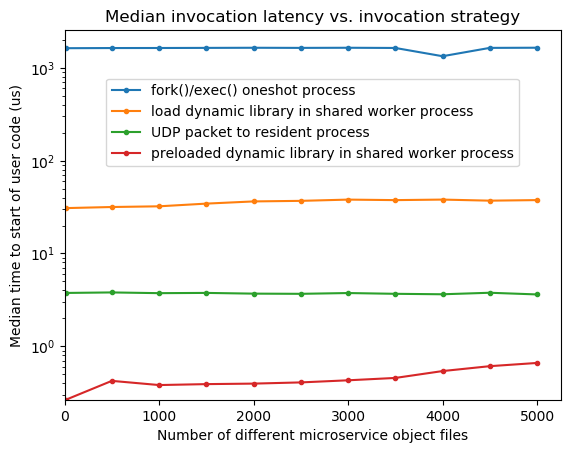
\includegraphics[width=\columnwidth]{figs/2018-02-02-motivation_numfuns-latency-reordered}
\caption{Median one-way invocation latencies for a microservice that does no work (note the log scale)}
\label{fig:motive}
\end{figure}

We conducted this benchmark and all other experiments on one 16-core socket of a
Linux 4.13.0 server equipped with 2.1-GHz Xeon E5-2683 Broadwell processors.  One
physical core was dedicated to a host-wide \textbf{dispatch process} that spools
requests and forwards them to 14 physical cores allocated to the microservices; the
remaining core was reserved for use by a thread that would communicate with the wider
serverless cluster management system.

Of course, consolidating multiple users' jobs into a single process requires
addressing the accompanying security challenges, and doing so in a way that
does not compromise our ambitious performance goals.
Fortunately, we can learn from two recently-published systems whose own demanding
performance requirements drove them to perform similar coalescing of traditionally
independent components:  NetBricks~\cite{Panda2016} is a network functions runtime
for providing programmable network capabilities; it is unique among this class of
systems for running the submitted functions in-process rather than in VMs.
Tock~\cite{Levy2017} is an embedded operating system that provides (in addition to a
more traditional process model) a type of lightweight application known as a capsule
that is embedded within the kernel and communicates with it using simple function
calls.  As their primary line of defense against untrusted code, both systems
leverage Rust~\cite{www-rustlang}, a new type-safe systems programming language.

Rust is a strongly-typed, compiled language that reprises C's abstention from a
heavyweight runtime.  Unlike many other modern systems languages, Rust is an
attractive choice when both performance and predictability are critical due to its
lack of a garbage collector.  Still, it manages to provide strong memory safety
guarantees by focusing on ``zero-cost abstractions'' (i.e., those that can be
compiled down to code whose safety is assured without runtime checks).  In
particular, safe Rust code is guaranteed to be free of null or dangling pointer
dereferences, invalid variable values (e.g., casts are checked and unions are
tagged), reads from uninitialized memory, mutations of non-\texttt{mut} data (roughly
the equivalent of C's \texttt{const}), and data races, among other
misbehaviors~\cite{www-rustlang-ub}.

We require each microservice to be written in Rust, which gives us many aspects of
the isolation we need:  It's difficult for microservices to crash the worker process,
since most segmentation faults are prevented, and runtime errors such as integer
overflow generate Rust panics that we can catch.  Microservices can't get references
to data that doesn't belong to them thanks to the variable and pointer initialization
rules.  However, given our performance goals, there is a significant aspect of the
required isolation that Rust doesn't provide:\ there is nothing to stop users from
monopolizing the CPU.  While it is true that other modern systems languages such as
Go~\cite{www-golang} and Erlang~\cite{www-erlang} include so-called ``green
threading'' (support for sharing a kernel thread among multiple tasks), this
multitasking is implemented cooperatively, so a task in a tight loop will never
yield.  To prevent this kind of behavior, our system needs to be preemptive.

The reader may be suspicious at the suggestion that we need to implement preemption,
given that operating systems have provided this functionality as a core service for
close to half a century.  However, we emphasize that our goals differ significantly
from those of an operating system:  An OS kernel avoids frequent preemption due to
the significant cost of rescheduling preempted work.  In contrast, the microservices
in our model are unapologetically lightweight and short-lived, and our system can
just kill any that time out.  Enforcing hard time limits is already an established
attribute of serverless systems, with the three large providers already limiting
microservices to minutes of runtime; we merely propose significantly reducing this
time budget.

Of course, the question remains of how the worker processes should implement
preemption, and at what granularity it is feasible to do so.  Hypothesizing that it
would be impossible to reliably preempt at finer granularity than a millisecond, we
performed a benchmark to assess the limits of the POSIX \texttt{setitimer()}
mechanism for repeatedly delivering \texttt{SIGALRM} signals separated by a custom
time interval.  We were surprised to find that, thanks to the HPETs (high precision
event timers) on modern CPUs, the signals were reliably delivered on time when we
requested intervals as small as 3 $\mu{}s$, even with timers set on all 14 worker
cores.
